\PassOptionsToPackage{unicode=true}{hyperref} % options for packages loaded elsewhere
\PassOptionsToPackage{hyphens}{url}
%
\documentclass[]{article}
\usepackage{lmodern}
\usepackage{amssymb,amsmath}
\usepackage{ifxetex,ifluatex}
\usepackage{fixltx2e} % provides \textsubscript
\ifnum 0\ifxetex 1\fi\ifluatex 1\fi=0 % if pdftex
  \usepackage[T1]{fontenc}
  \usepackage[utf8]{inputenc}
  \usepackage{textcomp} % provides euro and other symbols
\else % if luatex or xelatex
  \usepackage{unicode-math}
  \defaultfontfeatures{Ligatures=TeX,Scale=MatchLowercase}
\fi
% use upquote if available, for straight quotes in verbatim environments
\IfFileExists{upquote.sty}{\usepackage{upquote}}{}
% use microtype if available
\IfFileExists{microtype.sty}{%
\usepackage[]{microtype}
\UseMicrotypeSet[protrusion]{basicmath} % disable protrusion for tt fonts
}{}
\IfFileExists{parskip.sty}{%
\usepackage{parskip}
}{% else
\setlength{\parindent}{0pt}
\setlength{\parskip}{6pt plus 2pt minus 1pt}
}
\usepackage{hyperref}
\hypersetup{
            pdfborder={0 0 0},
            breaklinks=true}
\urlstyle{same}  % don't use monospace font for urls
\usepackage[margin=1in]{geometry}
\usepackage{color}
\usepackage{fancyvrb}
\newcommand{\VerbBar}{|}
\newcommand{\VERB}{\Verb[commandchars=\\\{\}]}
\DefineVerbatimEnvironment{Highlighting}{Verbatim}{commandchars=\\\{\}}
% Add ',fontsize=\small' for more characters per line
\usepackage{framed}
\definecolor{shadecolor}{RGB}{248,248,248}
\newenvironment{Shaded}{\begin{snugshade}}{\end{snugshade}}
\newcommand{\AlertTok}[1]{\textcolor[rgb]{0.94,0.16,0.16}{#1}}
\newcommand{\AnnotationTok}[1]{\textcolor[rgb]{0.56,0.35,0.01}{\textbf{\textit{#1}}}}
\newcommand{\AttributeTok}[1]{\textcolor[rgb]{0.77,0.63,0.00}{#1}}
\newcommand{\BaseNTok}[1]{\textcolor[rgb]{0.00,0.00,0.81}{#1}}
\newcommand{\BuiltInTok}[1]{#1}
\newcommand{\CharTok}[1]{\textcolor[rgb]{0.31,0.60,0.02}{#1}}
\newcommand{\CommentTok}[1]{\textcolor[rgb]{0.56,0.35,0.01}{\textit{#1}}}
\newcommand{\CommentVarTok}[1]{\textcolor[rgb]{0.56,0.35,0.01}{\textbf{\textit{#1}}}}
\newcommand{\ConstantTok}[1]{\textcolor[rgb]{0.00,0.00,0.00}{#1}}
\newcommand{\ControlFlowTok}[1]{\textcolor[rgb]{0.13,0.29,0.53}{\textbf{#1}}}
\newcommand{\DataTypeTok}[1]{\textcolor[rgb]{0.13,0.29,0.53}{#1}}
\newcommand{\DecValTok}[1]{\textcolor[rgb]{0.00,0.00,0.81}{#1}}
\newcommand{\DocumentationTok}[1]{\textcolor[rgb]{0.56,0.35,0.01}{\textbf{\textit{#1}}}}
\newcommand{\ErrorTok}[1]{\textcolor[rgb]{0.64,0.00,0.00}{\textbf{#1}}}
\newcommand{\ExtensionTok}[1]{#1}
\newcommand{\FloatTok}[1]{\textcolor[rgb]{0.00,0.00,0.81}{#1}}
\newcommand{\FunctionTok}[1]{\textcolor[rgb]{0.00,0.00,0.00}{#1}}
\newcommand{\ImportTok}[1]{#1}
\newcommand{\InformationTok}[1]{\textcolor[rgb]{0.56,0.35,0.01}{\textbf{\textit{#1}}}}
\newcommand{\KeywordTok}[1]{\textcolor[rgb]{0.13,0.29,0.53}{\textbf{#1}}}
\newcommand{\NormalTok}[1]{#1}
\newcommand{\OperatorTok}[1]{\textcolor[rgb]{0.81,0.36,0.00}{\textbf{#1}}}
\newcommand{\OtherTok}[1]{\textcolor[rgb]{0.56,0.35,0.01}{#1}}
\newcommand{\PreprocessorTok}[1]{\textcolor[rgb]{0.56,0.35,0.01}{\textit{#1}}}
\newcommand{\RegionMarkerTok}[1]{#1}
\newcommand{\SpecialCharTok}[1]{\textcolor[rgb]{0.00,0.00,0.00}{#1}}
\newcommand{\SpecialStringTok}[1]{\textcolor[rgb]{0.31,0.60,0.02}{#1}}
\newcommand{\StringTok}[1]{\textcolor[rgb]{0.31,0.60,0.02}{#1}}
\newcommand{\VariableTok}[1]{\textcolor[rgb]{0.00,0.00,0.00}{#1}}
\newcommand{\VerbatimStringTok}[1]{\textcolor[rgb]{0.31,0.60,0.02}{#1}}
\newcommand{\WarningTok}[1]{\textcolor[rgb]{0.56,0.35,0.01}{\textbf{\textit{#1}}}}
\usepackage{graphicx,grffile}
\makeatletter
\def\maxwidth{\ifdim\Gin@nat@width>\linewidth\linewidth\else\Gin@nat@width\fi}
\def\maxheight{\ifdim\Gin@nat@height>\textheight\textheight\else\Gin@nat@height\fi}
\makeatother
% Scale images if necessary, so that they will not overflow the page
% margins by default, and it is still possible to overwrite the defaults
% using explicit options in \includegraphics[width, height, ...]{}
\setkeys{Gin}{width=\maxwidth,height=\maxheight,keepaspectratio}
\setlength{\emergencystretch}{3em}  % prevent overfull lines
\providecommand{\tightlist}{%
  \setlength{\itemsep}{0pt}\setlength{\parskip}{0pt}}
\setcounter{secnumdepth}{0}
% Redefines (sub)paragraphs to behave more like sections
\ifx\paragraph\undefined\else
\let\oldparagraph\paragraph
\renewcommand{\paragraph}[1]{\oldparagraph{#1}\mbox{}}
\fi
\ifx\subparagraph\undefined\else
\let\oldsubparagraph\subparagraph
\renewcommand{\subparagraph}[1]{\oldsubparagraph{#1}\mbox{}}
\fi

% set default figure placement to htbp
\makeatletter
\def\fps@figure{htbp}
\makeatother


\author{}
\date{\vspace{-2.5em}}

\begin{document}

\hypertarget{introduction}{%
\subsection{1. Introduction:}\label{introduction}}

Visualization in three-dimensional (3D) space is a standard and critical
process for examining the complex structure of high dimensional data.
Stereo imaging technology can be adopted to enhance 3D representation of
any complex data, especially those consisting mostly of points and
lines. We illustrate the simple steps that are involved and strongly
encourage others to implement it in their own visualization software. To
facilitate its application, we have also created a new software that can
convert a regular 3D scatterplot or network figure to a stereo
image(Liu, Singh, and Zheng 2020)

\hypertarget{concept}{%
\subsection{2. Concept:}\label{concept}}

When 2D-image of original data and the slightly rotated data are viewed
side by side a 3D illusion is created due to two perspectives of the
same object.

The original set of coordinates \((X, Y, Z)\) can be rotated
(counter-clockwise direction) by an angle \(\theta\) along Y-axis using
the rotation matrix \(R_y (\theta)\). The new set of coordinates is
obtained as

\begin{figure}
\centering
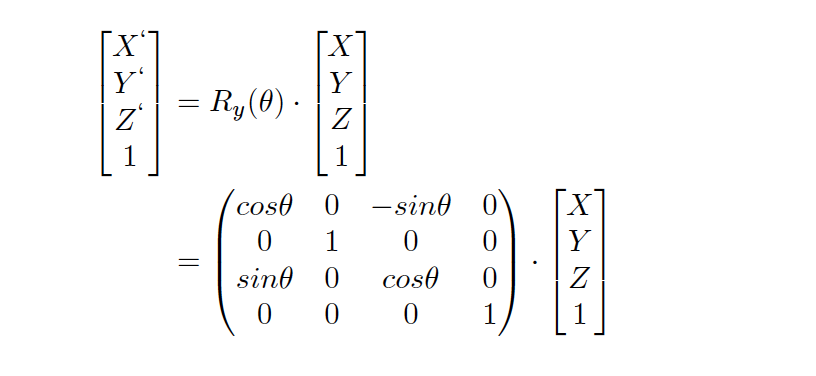
\includegraphics{./equation.png}
\caption{""}
\end{figure}

\hypertarget{availability-and-installation}{%
\subsection{3. Availability and
Installation}\label{availability-and-installation}}

The development version of \texttt{Stereo3D} package is available at
\url{https://github.com/bioinfoDZ/Stereo3D} and can be installed as

\begin{Shaded}
\begin{Highlighting}[]
\CommentTok{# install.packages("devtools")}
\NormalTok{devtools}\OperatorTok{::}\KeywordTok{install_github}\NormalTok{(}\StringTok{"bioinfoDZ/Stereo3D"}\NormalTok{,}\DataTypeTok{build_vignettes =} \OtherTok{FALSE}\NormalTok{ )}
\end{Highlighting}
\end{Shaded}

\hypertarget{functions}{%
\subsection{4. Functions}\label{functions}}

\hypertarget{stereo3d}{%
\subsubsection{4.1 Stereo3D}\label{stereo3d}}

\#\#\#\#\textbf{Description} Create Stereoscopic 3D image of the given
data.

\#\#\#\#\textbf{Usage}
\texttt{Stereo3D(data\_file=sample\_data\_file,\ stereo\_angle=5,\ distance=0,\ connection\_file=connection\_fileNam)}

\#\#\#\#\textbf{Arguments } - \texttt{data\_file}: A tab seperated file
with \texttt{".tsv"} extension and having five columns (\texttt{index},
\texttt{X}, \texttt{Y}, \texttt{Z} and \texttt{Color}) of the data.
Where, \texttt{X}, \texttt{Y} and \texttt{Z} represent cordinates of a
datapoint, \texttt{Color} is the label of the given data point and
\texttt{index} clolumn have the index information of the datapoints. -
\texttt{stereo\_angle}: angle by which 3D data to be rotated along
Y-axis. \texttt{Default:\ 5\ degree} - \texttt{distance}: Distance or
gap between the two stereo images. - \texttt{connection\_file}: A tab
seperated file (optional). Where, \texttt{first} and \texttt{second}
column has indices of start and end points (from \texttt{data\_file}) of
a connection respectively.

\#\#\#\#\textbf{Details} The dataset is rotatated by a given angle along
the Y-axis and a Stereoscopic 3D scatter plot image is created.

\#\#\#\#\textbf{Value}

\begin{itemize}
\tightlist
\item
  Create Stereoscopic 3D plot with
  \texttt{input\ data\ filename\ prefix} and \texttt{\_Stereo.pdf}
  extention.
\item
  Interactive 3D plot for the above image pops up, which can be zoomed
  and rotated by draging the mouse.
\end{itemize}

\#\#\#\#\textbf{Examples}

\begin{verbatim}
> connection_fileName=system.file("extdata", "connection_file.tsv",
package = "Stereo3D", mustWork = TRUE)
> sample_data_file=system.file("extdata", "sample_3D_data.tsv",
package = "Stereo3D", mustWork = TRUE)

> Stereo3D(data_file=sample_data_file, stereo_angle=5, distance=0,
connection_file=connection_fileName) # dataset stereo image is created
and saved as "sample_3D_data_Stereo.pdf", another interactive 3D image also pops-up.
\end{verbatim}

\hypertarget{output}{%
\paragraph{Output}\label{output}}

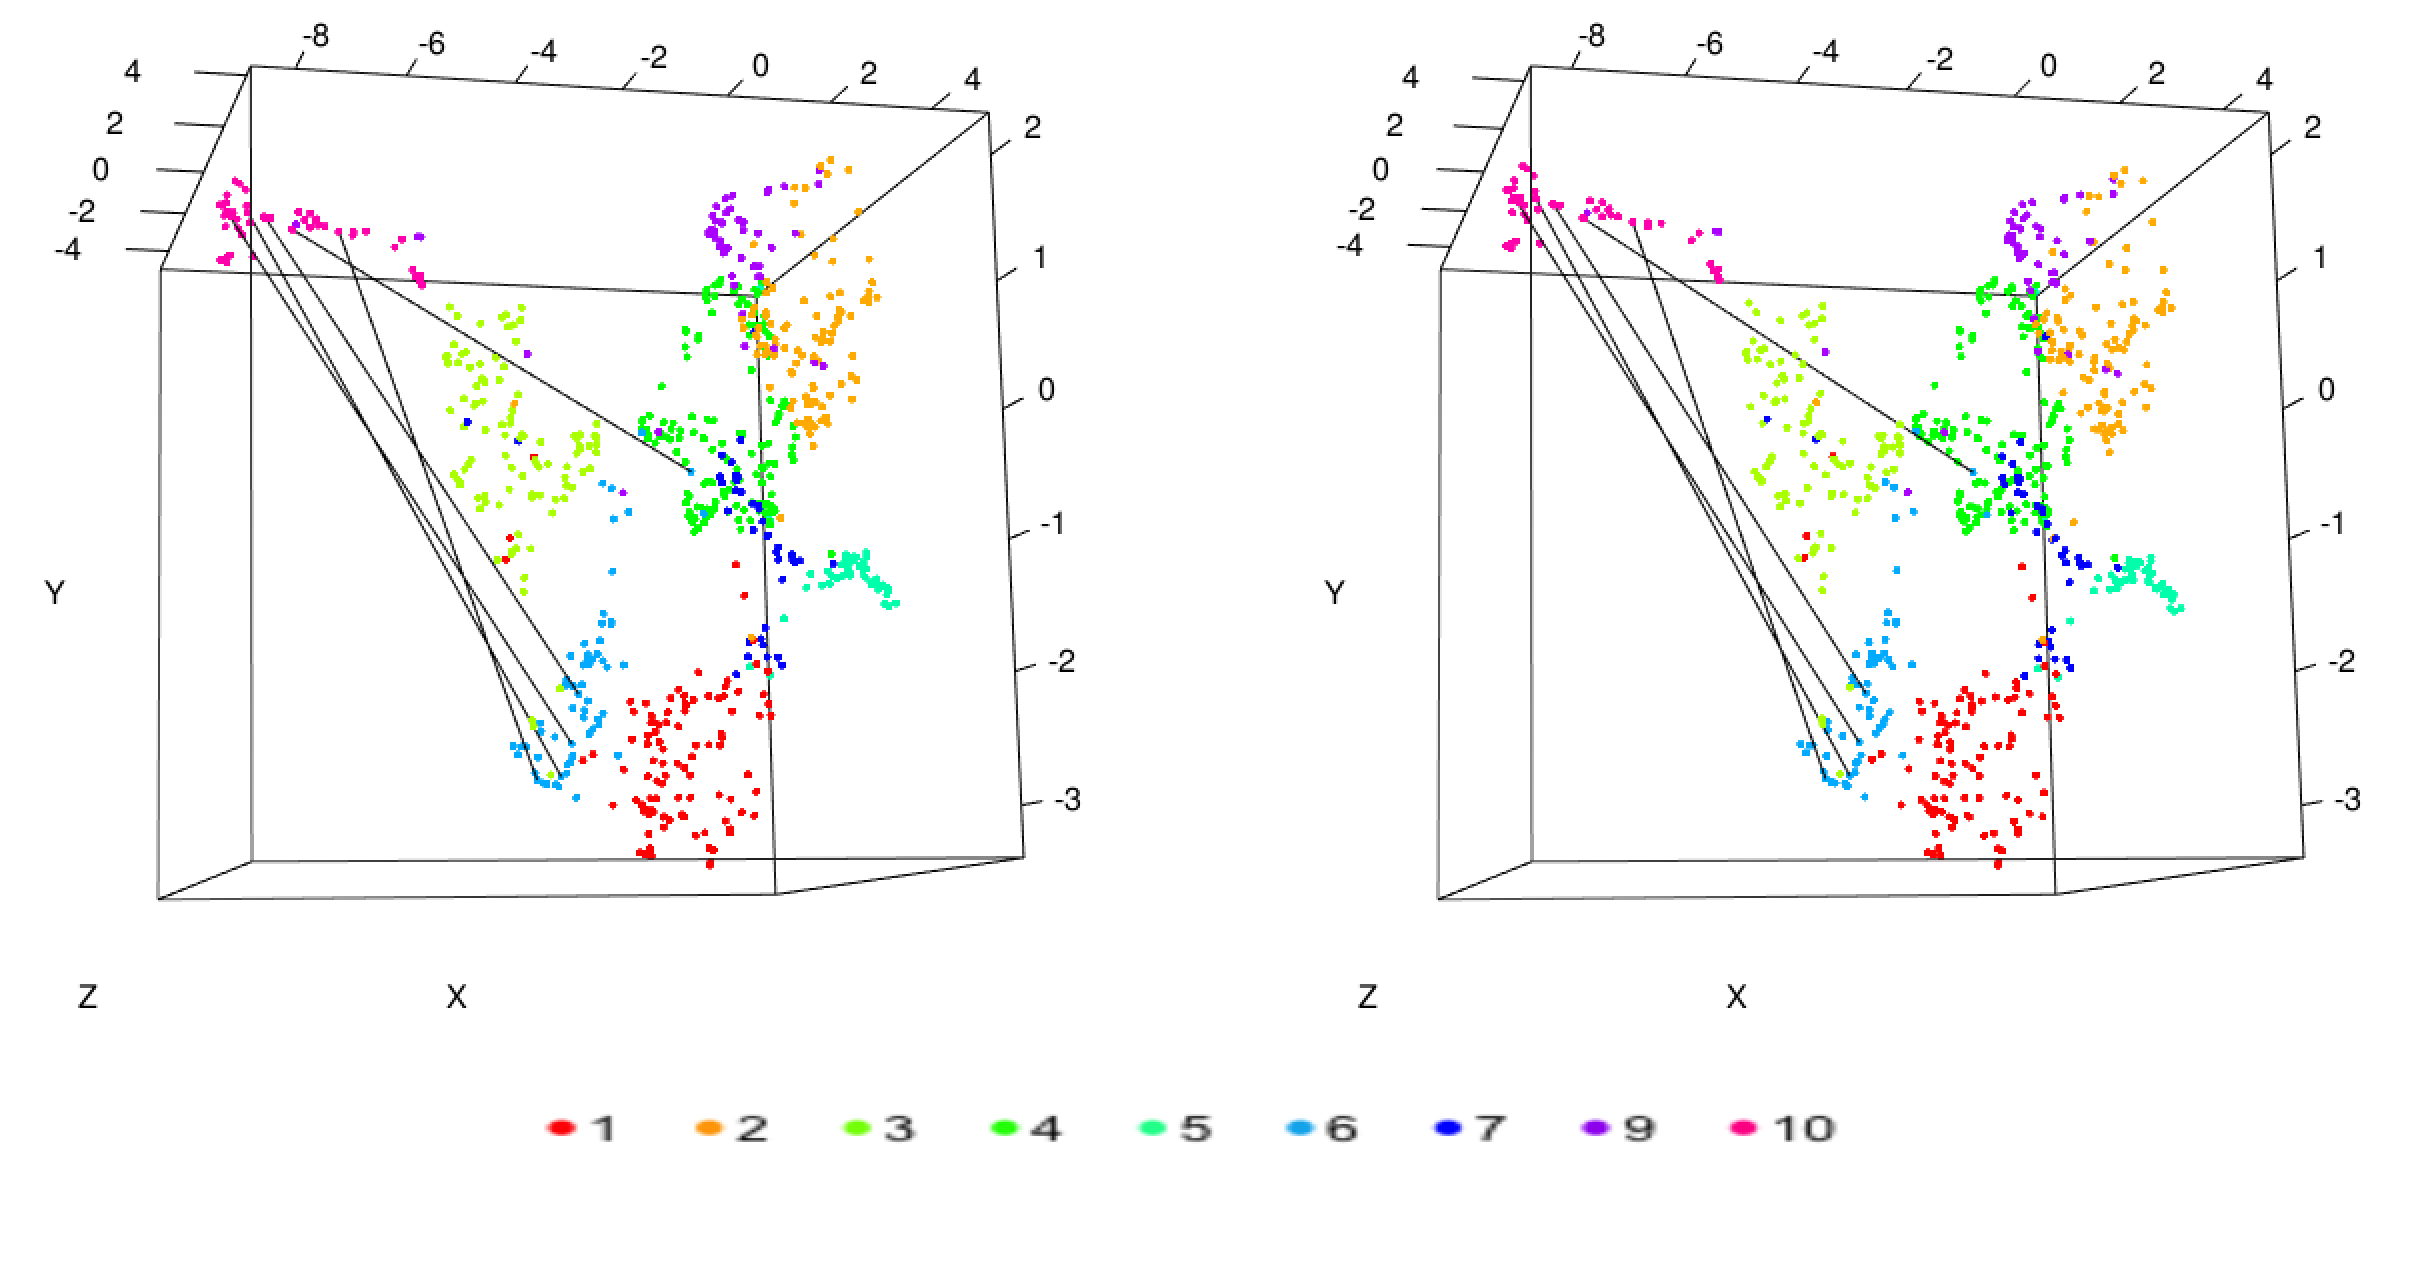
\includegraphics{./sample.png} 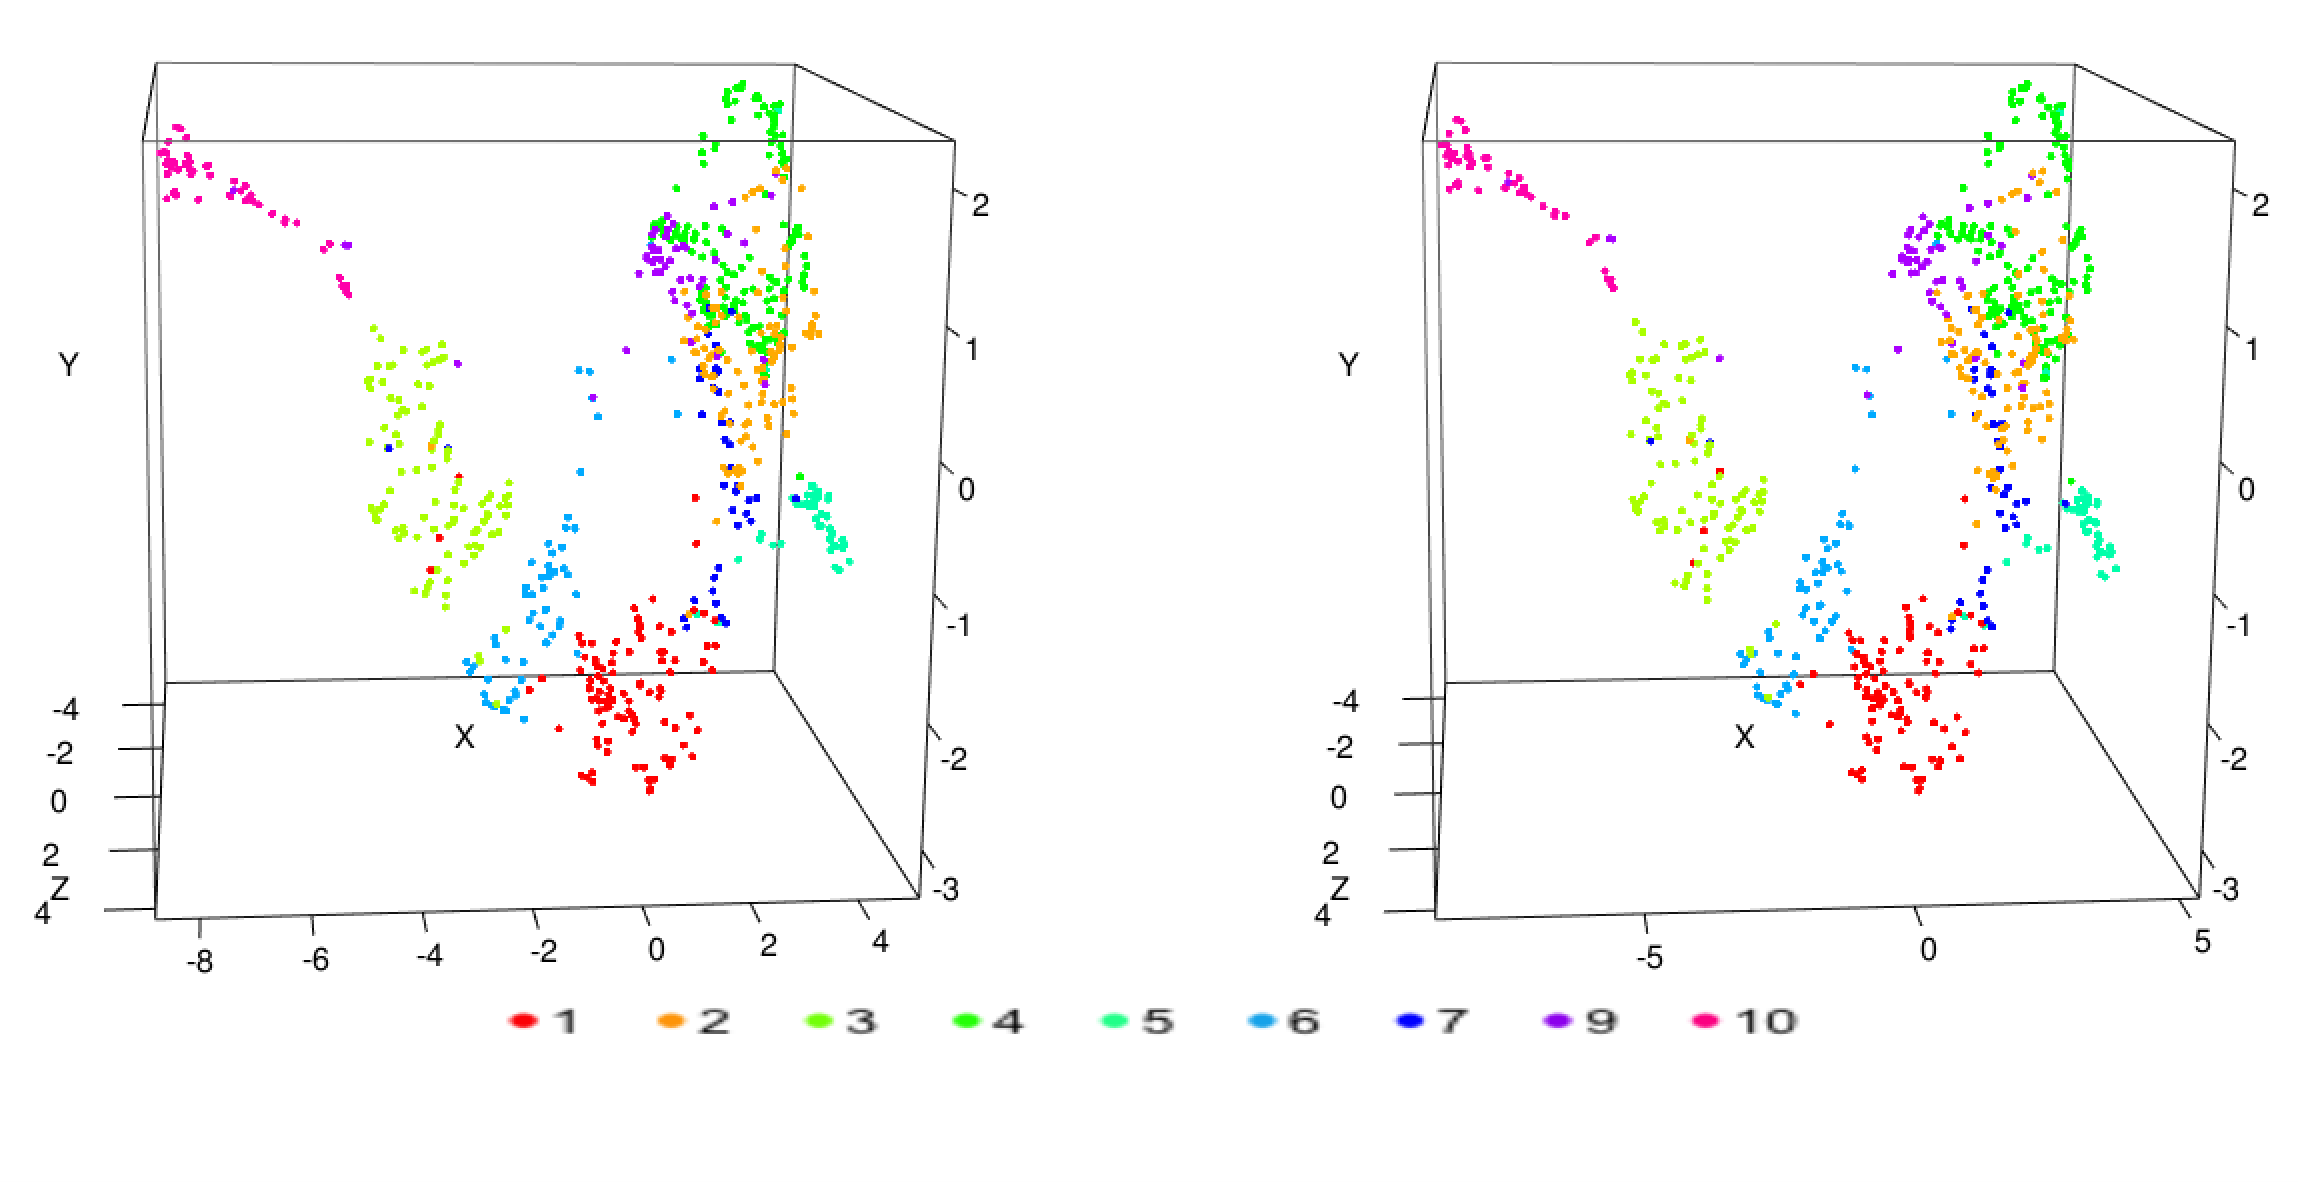
\includegraphics{./sample_scatter.png}

\begin{figure}
\centering
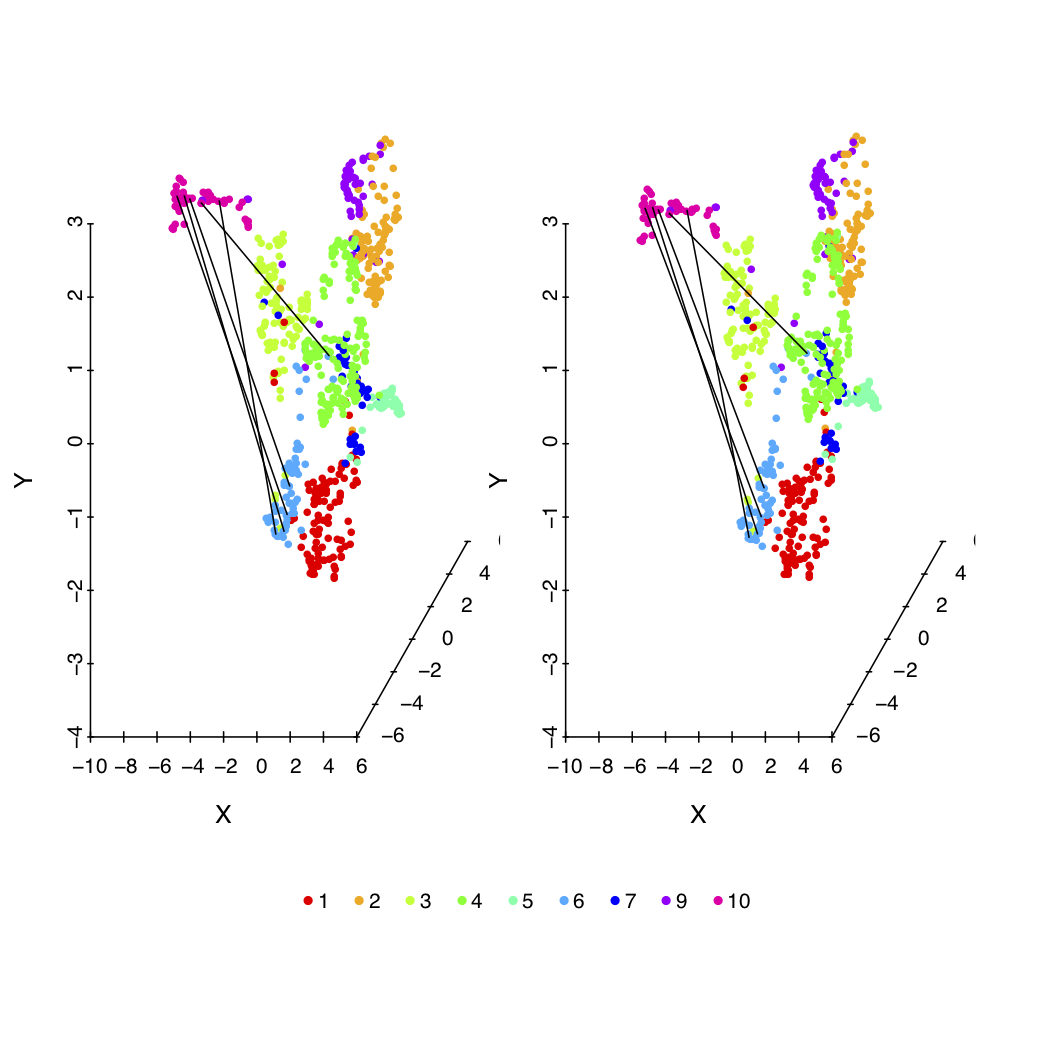
\includegraphics{./sample_3D_data_Stereo_net.png}
\caption{``Output: Sterio Image''}
\end{figure}

\hypertarget{refs}{}
\leavevmode\hypertarget{ref-10.1093ux2fbioinformaticsux2fbtaa521}{}%
Liu, Yang, Vinod Kumar Singh, and Deyou Zheng. 2020. ``Stereo3D: using
stereo images to enrich 3D visualization.'' \emph{Bioinformatics}, May.
\url{https://doi.org/10.1093/bioinformatics/btaa521}.

\end{document}
